%%
%% This is file `sample-sigconf.tex',
%% generated with the docstrip utility.
%%
%% The original source files were:
%%
%% samples.dtx  (with options: `sigconf')
%% 
%% IMPORTANT NOTICE:
%% 
%% For the copyright see the source file.
%% 
%% Any modified versions of this file must be renamed
%% with new filenames distinct from sample-sigconf.tex.
%% 
%% For distribution of the original source see the terms
%% for copying and modification in the file samples.dtx.
%% 
%% This generated file may be distributed as long as the
%% original source files, as listed above, are part of the
%% same distribution. (The sources need not necessarily be
%% in the same archive or directory.)
%%
%%
%% Commands for TeXCount
%TC:macro \cite [option:text,text]
%TC:macro \citep [option:text,text]
%TC:macro \citet [option:text,text]
%TC:envir table 0 1
%TC:envir table* 0 1
%TC:envir tabular [ignore] word
%TC:envir displaymath 0 word
%TC:envir math 0 word
%TC:envir comment 0 0
%%
%%
%% The first command in your LaTeX source must be the \documentclass command.
\documentclass[sigconf,authordraft]{acmart}

\usepackage[binary-units]{siunitx}

% Visible TODO notes
\newcommand{\todo}[1]{\textbf{\textsc{\textcolor{red}{(TODO: #1)}}}}

%%
%% \BibTeX command to typeset BibTeX logo in the docs
\AtBeginDocument{%
  \providecommand\BibTeX{{%
    \normalfont B\kern-0.5em{\scshape i\kern-0.25em b}\kern-0.8em\TeX}}}

%% Rights management information.  This information is sent to you
%% when you complete the rights form.  These commands have SAMPLE
%% values in them; it is your responsibility as an author to replace
%% the commands and values with those provided to you when you
%% complete the rights form.
\setcopyright{acmcopyright}
\copyrightyear{2021}
\acmYear{2021}
\acmDOI{10.1145/1122445.1122456}

%% These commands are for a PROCEEDINGS abstract or paper.
\acmConference[NICE '21]{Neuro-inspired Computational Elements Workshop}{March 28--April 1, 2021}{San Antonio, TX}
\acmBooktitle{NICE '21: Proceedings of the Neuro-inspired Computational Elements Workshop}
\acmPrice{15.00}
\acmISBN{9978-1-4503-9559-5}


%%
%% Submission ID.
%% Use this when submitting an article to a sponsored event. You'll
%% receive a unique submission ID from the organizers
%% of the event, and this ID should be used as the parameter to this command.
%%\acmSubmissionID{123-A56-BU3}

%%
%% The majority of ACM publications use numbered citations and
%% references.  The command \citestyle{authoryear} switches to the
%% "author year" style.
%%
%% If you are preparing content for an event
%% sponsored by ACM SIGGRAPH, you must use the "author year" style of
%% citations and references.
%% Uncommenting
%% the next command will enable that style.
%%\citestyle{acmauthoryear}

%%
%% end of the preamble, start of the body of the document source.
\begin{document}

%%
%% The "title" command has an optional parameter,
%% allowing the author to define a "short title" to be used in page headers.
\title{Efficient GPU training of LSNNs using eProp}

%%
%% The "author" command and its associated commands are used to define
%% the authors and their affiliations.
%% Of note is the shared affiliation of the first two authors, and the
%% "authornote" and "authornotemark" commands
%% used to denote shared contribution to the research.
\author{James C Knight}
\email{J.C.Knight@sussex.ac.uk}
\orcid{0000-0003-0577-0074}
\affiliation{%
  \institution{University of Sussex}
  \department{School of Engineering and Informatics}
  \city{Brighton}
  \country{United Kingdom}
}

\author{Thomas Nowotny}
\email{T.Nowotny@sussex.ac.uk}
\orcid{0000-0002-4451-915X}
\affiliation{%
  \institution{University of Sussex}
  \department{School of Engineering and Informatics}
  \city{Brighton}
  \country{United Kingdom}
}
%%
%% By default, the full list of authors will be used in the page
%% headers. Often, this list is too long, and will overlap
%% other information printed in the page headers. This command allows
%% the author to define a more concise list
%% of authors' names for this purpose.
\renewcommand{\shortauthors}{Knight and Nowotny}

%%
%% The abstract is a short summary of the work to be presented in the
%% article.
\begin{abstract}
    Taking inspiration from machine learning libraries -- where techniques such as parallel batch training minimise latency and maximise GPU occupancy -- as well as our previous research on efficiently simulating Spiking Neural Networks~(SNNs) on GPUs for computational neuroscience, we have extended our GeNN SNN simulator to enable spiske-based machine learning research on general purpose hardware.
    We demonstrate that SNN classifiers implemented using GeNN and trained using the eProp learning rule can provide comparable performance to those trained using Back Propagation Through Time and show that the latency and energy usage of our SNN classifiers is up to $7\times$ lower than an LSTM running on the same GPU hardware.
\end{abstract}

%%
%% The code below is generated by the tool at http://dl.acm.org/ccs.cfm.
%% Please copy and paste the code instead of the example below.
%%
\begin{CCSXML}
<ccs2012>
   <concept>
       <concept_id>10010147.10010257.10010293.10011809</concept_id>
       <concept_desc>Computing methodologies~Bio-inspired approaches</concept_desc>
       <concept_significance>300</concept_significance>
       </concept>
   <concept>
       <concept_id>10010147.10010257.10010258.10010259</concept_id>
       <concept_desc>Computing methodologies~Supervised learning</concept_desc>
       <concept_significance>300</concept_significance>
       </concept>
   <concept>
       <concept_id>10010147.10010169.10010170.10010173</concept_id>
       <concept_desc>Computing methodologies~Vector / streaming algorithms</concept_desc>
       <concept_significance>300</concept_significance>
       </concept>
 </ccs2012>
\end{CCSXML}

\ccsdesc[300]{Computing methodologies~Bio-inspired approaches}
\ccsdesc[300]{Computing methodologies~Supervised learning}
\ccsdesc[300]{Computing methodologies~Vector / streaming algorithms}

%%
%% Keywords. The author(s) should pick words that accurately describe
%% the work being presented. Separate the keywords with commas.
\keywords{datasets, neural networks, gaze detection, text tagging}

%%
%% This command processes the author and affiliation and title
%% information and builds the first part of the formatted document.
\maketitle

\section{Introduction}
In recent years, several new techniques for directly training spiking neural networks~(SNNs) have been developed.
One approach is to replace the non-differentiable `transfer function' of a spiking neuron with a differentiable surrogate function~\citep{Bohte2011,Bellec2018,Zenke2021a}, allowing SNNs to be trained with the same algorithms used to train rate-based Recurrent Neural Network~(RNNs) such as Back Propagation Through Time~(BPTT).
While BPTT is computationally efficient -- because it requires gradients to be stored during the forward pass in order for them to be applied during a backward pass -- it has a memory requirement which grows with time preventing it from being applied to long input sequences or used online.
RTRL~\citep{Williams1989} is an alternative `forward mode' algorithm for training RNNs but, in its general form, it is too computationally expensive to be practical.
However, if the gradients flowing through the `explicit' recurrent connections are ignored and only those flowing through the `implicit' recurrence represented by the dynamics of individual neurons is considered, much more computationally tractable learning rules can be derived~\citep{Zenke2021}.
Learning rules of this sort include SuperSpike~\citep{Zenke2018}, eProp~\citep{Bellec2018} and Decolle~\citep{Kaiser2020}.
\todo{some background on spike-time based learning}
However, in order to apply new spike-based machine learning techniques to larger models and data-sets as well as prototyping algorithms for neuromorphic hardware~\citep{Davies2018,Furber2014,Merolla2014}, new tools are required which can efficiently simulate SNNs on existing hardware. 
The development of efficient SNN simulators has been a key area of computational neuroscience research for several decades~\citep{carnevale2006neuron, Gewaltig2007, Golosio2021, Akar2019,Yavuz2016} but, these simulators \todo{more}, making them ill-suited for spike-based machine learning research.
As such, many ML researchers have chosen to build libraries~\citep{norse2021, SpikingJelly, eshraghian2021training,Hazan2018} on top of more familiar tools such as PyTorch.
However, while libraries like PyTorch are highly-optimised for rate-based models, they does not take advantage of the spatio-temporal sparsity of SNNs which have the potential to enable massive computational savings over rate-based networks~\citep{Yin2021}.

While our GeNN simulator~\citep{Yavuz2016,Knight2018,Knight2021} was originally developed for Computational Neuroscience research, its longstanding focus on flexibility and its targeting of GPU accelerators make it well-suited to the needs of spike-based ML.
\todo{talk about additions to GeNN}
Here we demonstrate this by training SNN classifiers on the Spiking Heidelberg Digits~\citep{Cramer2020} and the Spiking Sequential MNIST~\citep{Plank2021} datasets.
In section~\ref{sec:accuracy} we compare the trained performance of these classifiers to those trained using BPTT, in section~\ref{sec:training_time} we compare the time taken to train these models and in section~\ref{sec:inference_time} we compare the latency and energy usage of our SNN classifiers to LSTMs running on the same GPU hardware.

%Specialised neuromorphic hardware~\todo{cite usual suspects} can be used to implement SNNs very efficiently but, while some consensus is beginning to emerge on the theoretical framework within which biological learning may operate, casting algorithms into hardware always results in a game of catch-up with even the most flexible current neuromorphic systems being capable of implementing only very limited versions of the latest online learning rules~\todo{cite garrick}.

\begin{figure*}[t]
  \centering
  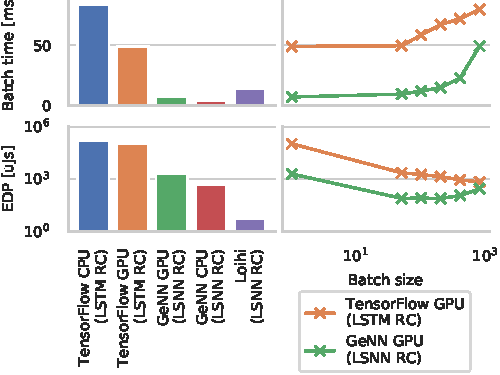
\includegraphics{figures/lstm_vs_genn.pdf}
  \caption{1907 Franklin Model D roadster. Photograph by Harris \&
    Ewing, Inc. [Public domain], via Wikimedia
    Commons. (\url{https://goo.gl/VLCRBB}).}
  \label{fig:lstm_vs_genn}
\end{figure*}

\begin{figure}[t]
  \centering
  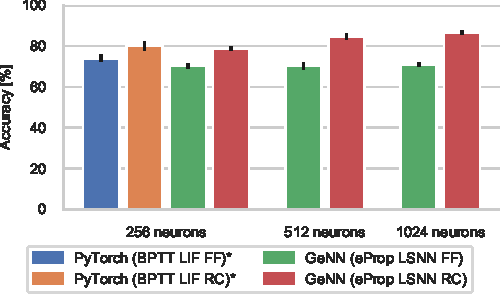
\includegraphics{figures/shd_performance.pdf}
  \caption{Comparison of performance on Spiking Heidelberg Digits dataset of LSNNs trained with eProp using GeNN and SNNs trained with BPTT using PyTorch~\citep{Zenke2021a}.
  Bars signify the mean and error bars the standard deviation over 5~(GeNN) and 10~(PyTorch) simulations.}
  \label{fig:shd_performance}
\end{figure}

\begin{figure}[t]
  \centering
  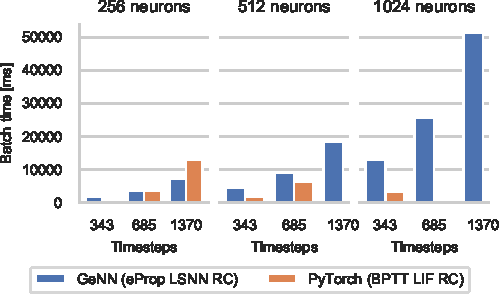
\includegraphics{figures/training_time.pdf}
  \caption{Comparison of training times on Spiking Heidelberg Digits dataset of LSNNs trained with eProp using GeNN and SNNs trained with BPTT using PyTorch. All experiments are performed on a \SI{12}{\giga\byte} Titan V GPU. The input spike trains are binned into different numbers of timesteps. Missing bars indicate that GPU had insufficient memory for experiment.}
  \label{fig:training_time}
\end{figure}

\section{Results}
We trained LSNNs of various sizes with feedforward and recurrent connectivity on the Spiking Heidelberg Digits~(SHD)~\citep{Cramer2020} and spiking sequential MNIST~\citep{Plank2021} datasets using eProp with the default parameters employed by \citet{Bellec2020}.

\subsection{Accuracy}
\label{sec:accuracy}
In figure~\ref{fig:shd_performance} we compare the performance of our models trained on the SHD dataset with results obtained by \citet{Zenke2021a} using BPTT.
There is no significant \todo{suitable significance test?} different between the performance of the \num{256} neuron models and, because the reduced memory requirement of eProp allow larger models to be trained, we show that the performance can be significantly improved by increasing the number of neurons to \num{512}.

\subsection{Training time}
\label{sec:training_time}
While being able to train networks with high classification accuracy is important, training also needs to fast.
In figure~\ref{fig:training_time} we compare the time taken to train recurrent LSNNs using eProp with GeNN against recurrent LIF networks training using BPTT with PyTorch.
\todo{analysis}

\subsection{Inference time}
\label{sec:inference_time}
In figure~\ref{fig:lstm_vs_genn}, we compare the inference time and energy delay products~\todo{cite} of LSNNs simulated using GeNN against LSTM models running on the same hardware~\citep{Plank2021} as well as LSNNs running on the Loihi neuromorphic system~\citep{Davies2018}.
On the same Titan V GPU, LSNNs are faster than LSTMs and have a lower EDP across all batch sizes.
Compared to inference using LSTMs, LSNN inference has a much lower arithmetic intensity meaning that, at batch size 1, not only is the CPU code generated by GeNN faster than TensorFlow running on CPU but it is also faster than GeNN running on GPU.
Finally, although LSNN inference on Loihi has a much lower Energy-Delay Prodyct, inference on both GPU and CPU using GeNN has lower latency.

\section{Future work}
\todo{EventProp, convolutional networks, deeper networks}

\section{Conclusions}
By adding additional functionality aimed at accelerating spike-based machine learning workflows to our GeNN simulator, we have demonstrated that training using `forward-mode' learning rules like eProp can not only result in competitive accuracy in classification tasks but also allow  larger models to be trained on longer input sequences than is possible when using BPTT.
Finally we demonstrate that, by exploiting temporal sparsity, standard CPU and GPU hardware can perform inference faster and with less energy using LSNNs than it can using standard LSTM models.

%%
%% The acknowledgments section is defined using the "acks" environment
%% (and NOT an unnumbered section). This ensures the proper
%% identification of the section in the article metadata, and the
%% consistent spelling of the heading.
\begin{acks}
To Robert, for the bagels and explaining CMYK and color spaces.
\end{acks}

%%
%% The next two lines define the bibliography style to be used, and
%% the bibliography file.
\bibliographystyle{ACM-Reference-Format}
\bibliography{eprop}

\end{document}
\endinput
%%
%% End of file `sample-sigconf.tex'.
